% this TeX file provides an awesome example of how TeX will make super 
% awesome tables, at the cost of your of what happens when you try to make a
% table that is very complicated.
\documentclass[11pt]{article}

% Use wide margins, but not quite so wide as fullpage.sty
\marginparwidth 0.5in 
\oddsidemargin 0.25in 
\evensidemargin 0.25in 
\marginparsep 0.25in
\topmargin 0.25in
\textwidth 6in
\textheight 8in
% That's about enough definitions

% language input
\usepackage[utf8]{inputenc}
% multirow allows you to combine rows in columns
\usepackage{multirow}
% tabularx allows manual tweaking of column width
\usepackage{tabularx}
% insert images
\usepackage{graphicx}
\usepackage{float}
\graphicspath{ {images/} }

\begin{document}
% this is an alternate method of creating a title
%\hfill\vbox{\hbox{Gius, Mark}
%       \hbox{Cpe 456, Section 01}  
%       \hbox{Lab 1}    
%       \hbox{\today}}\par
%
%\bigskip
%\bigskip
\author{Vandré Leal Cândido}
\title{Wireshark Lab: HTTP v6.1}
\maketitle

% 1. The Basic HTTP GET/response interaction
\section{The Basic HTTP GET/response interaction}

\begin{figure}[H]
\centering
\caption{Request (Section 1)}
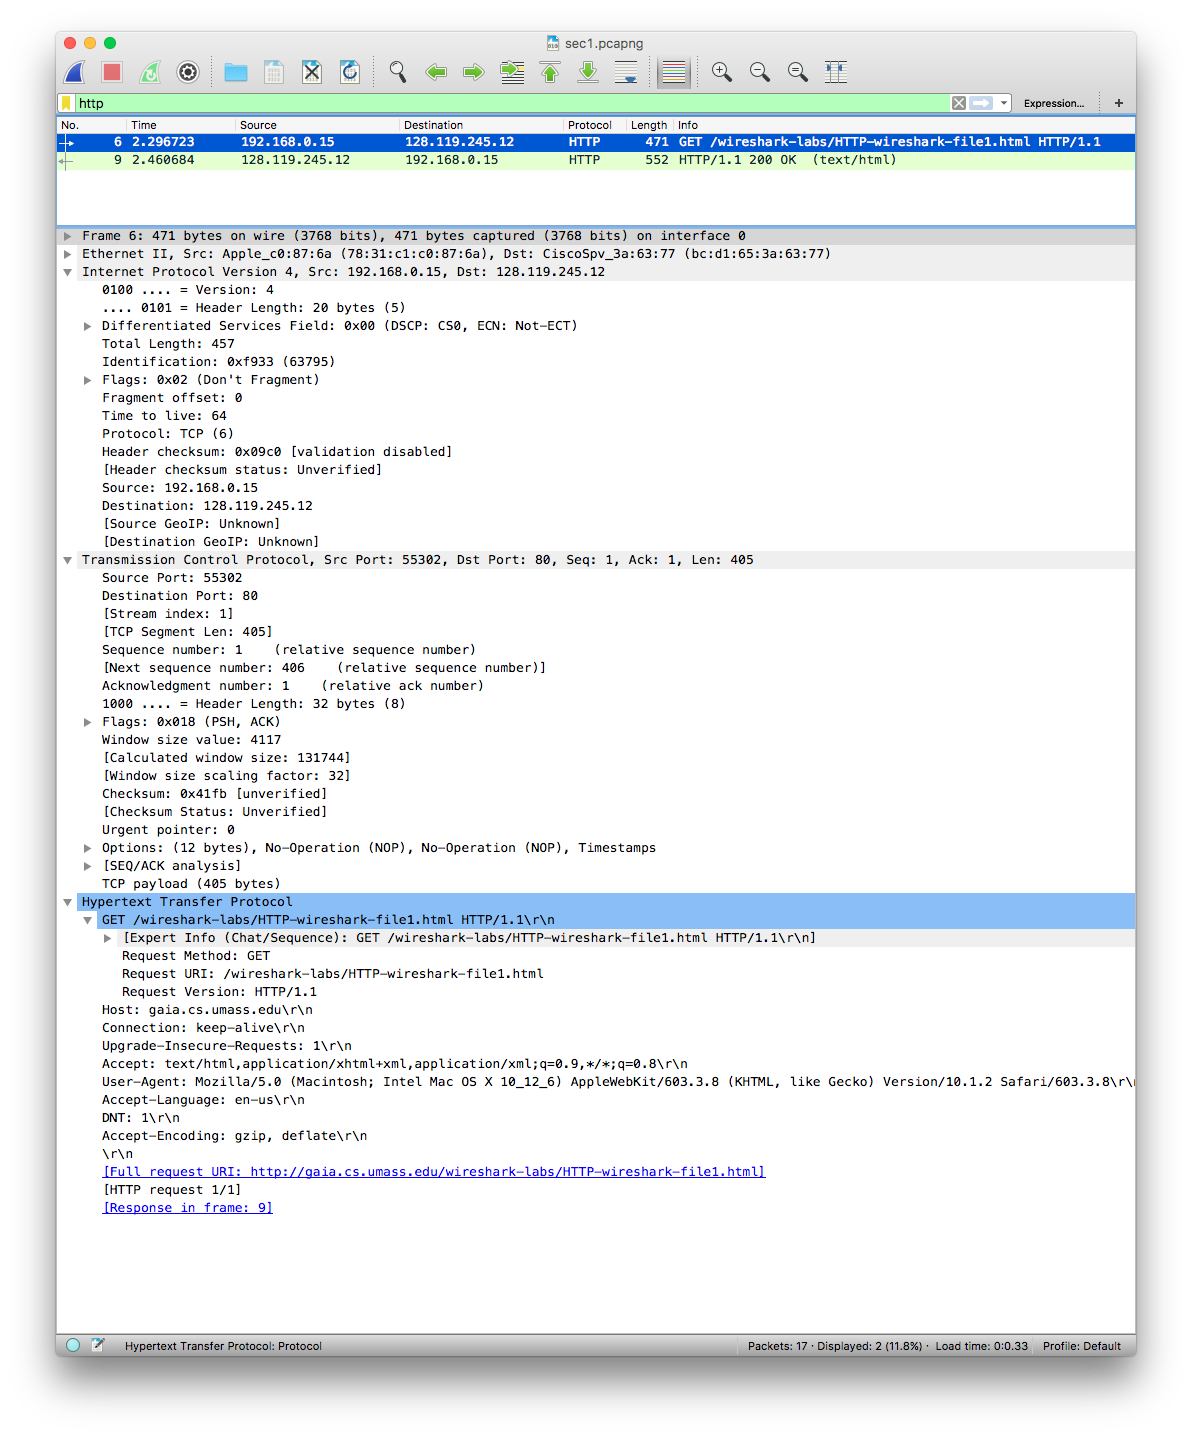
\includegraphics[width=\textwidth]{01-request}
\end{figure}

\begin{figure}[H]
\centering
\caption{Response (Section 1)}
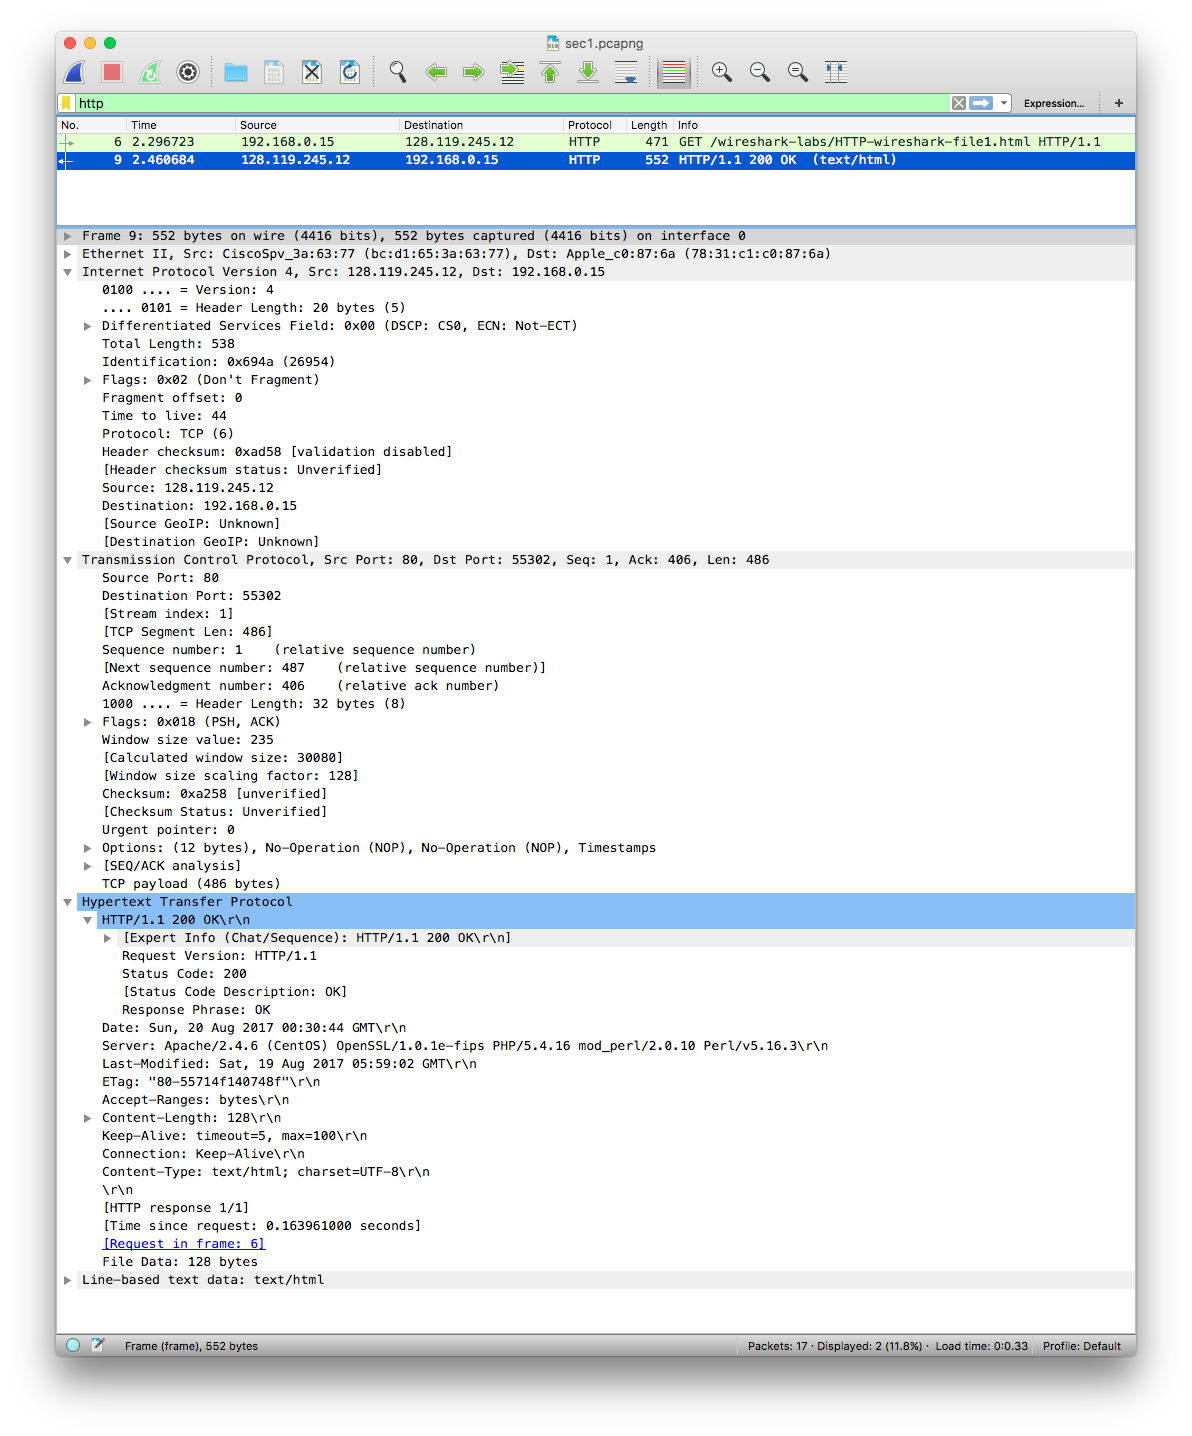
\includegraphics[width=\textwidth]{01-response}
\end{figure}

\pagebreak

\begin{itemize}
	\setlength\itemsep{.5cm}

	\item
		\textit{Is your browser running HTTP version 1.0 or 1.1? What version of HTTP is the server running?}
		\par Both browser and server use HTTP version 1.1.
	
	\item
		\textit{What languages (if any) does your browser indicate that it can accept to the server?}
		\par Only US English. [Accept-Language: en-us]
	
	\item
		\textit{What is the IP address of your computer? Of the gaia.cs.umass.edu server?}
		\par Local IP address: 192.168.0.15 / gaia.cs.umass.edu: 128.119.245.12.
		
	\item
		\textit{What is the status code returned from the server to your browser?}
		\par The status code returned is 200 [OK].
		
	\item
		\textit{When was the HTML file that you are retrieving last modified at the server?}
		\par The HTML file was Last-Modified: Sat, 19 Aug 2017 05:59:02 GMT.
		
	\item
		\textit{How many bytes of content are being returned to your browser?}
		\par 128 bytes of content are being returned. [Content-Length: 128]
		
	\item
		\textit{By inspecting the raw data in the packet content window, do you see any headers within
the data that are not displayed in the packet-listing window? If so, name one.}
		\par No, all headers can be found in the raw data.
	
\end{itemize}

\pagebreak

% 2. The HTTP CONDITIONAL GET/response interaction
\section{The HTTP CONDITIONAL GET/response interaction}

\begin{itemize}
	\setlength\itemsep{.5cm}

	\item
		\textit{Inspect the contents of the first HTTP GET request from your browser to the server. Do
you see an “IF-MODIFIED-SINCE” line in the HTTP GET?}
		\par No, there isn't an “IF-MODIFIED-SINCE” line in the first HTTP GET.
		
		\begin{figure}[H]
		\centering
		\caption{First Request (Section 2)}
		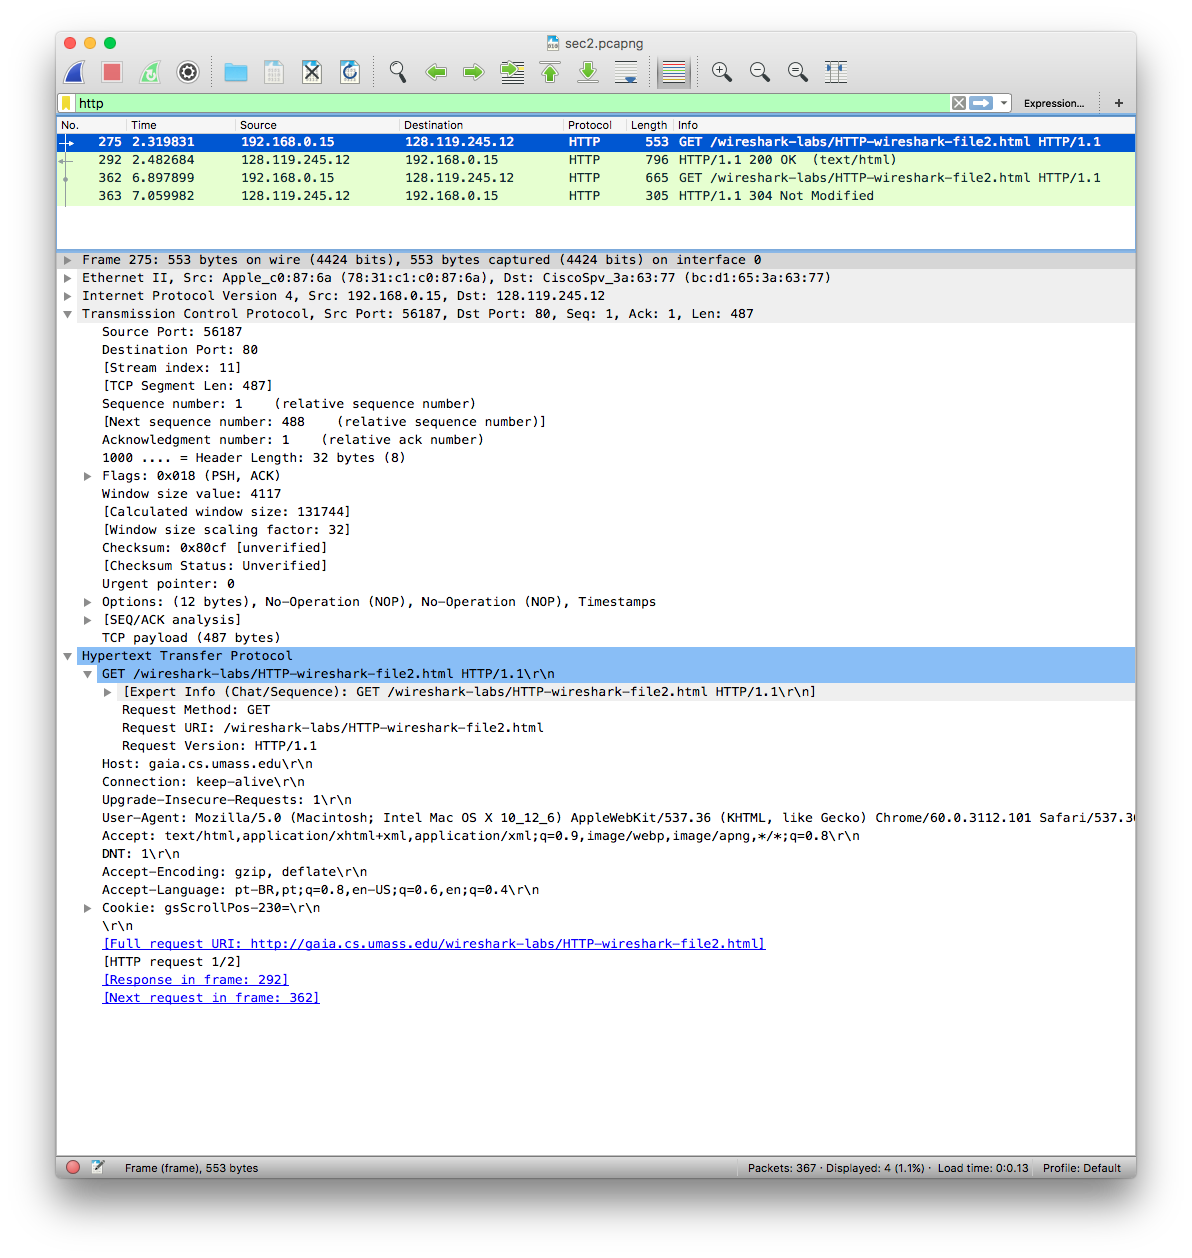
\includegraphics[width=\textwidth]{02-request_1}
		\end{figure}
		
	\item
		\textit{Inspect the contents of the server response. Did the server explicitly return the contents
of the file? How can you tell?}
		\par Yes, the server explicitly returned the contents of the HTML file. The content is included in `Line-based text data: text/html'.
		
		\begin{figure}[H]
		\centering
		\caption{First Response (Section 2)}
		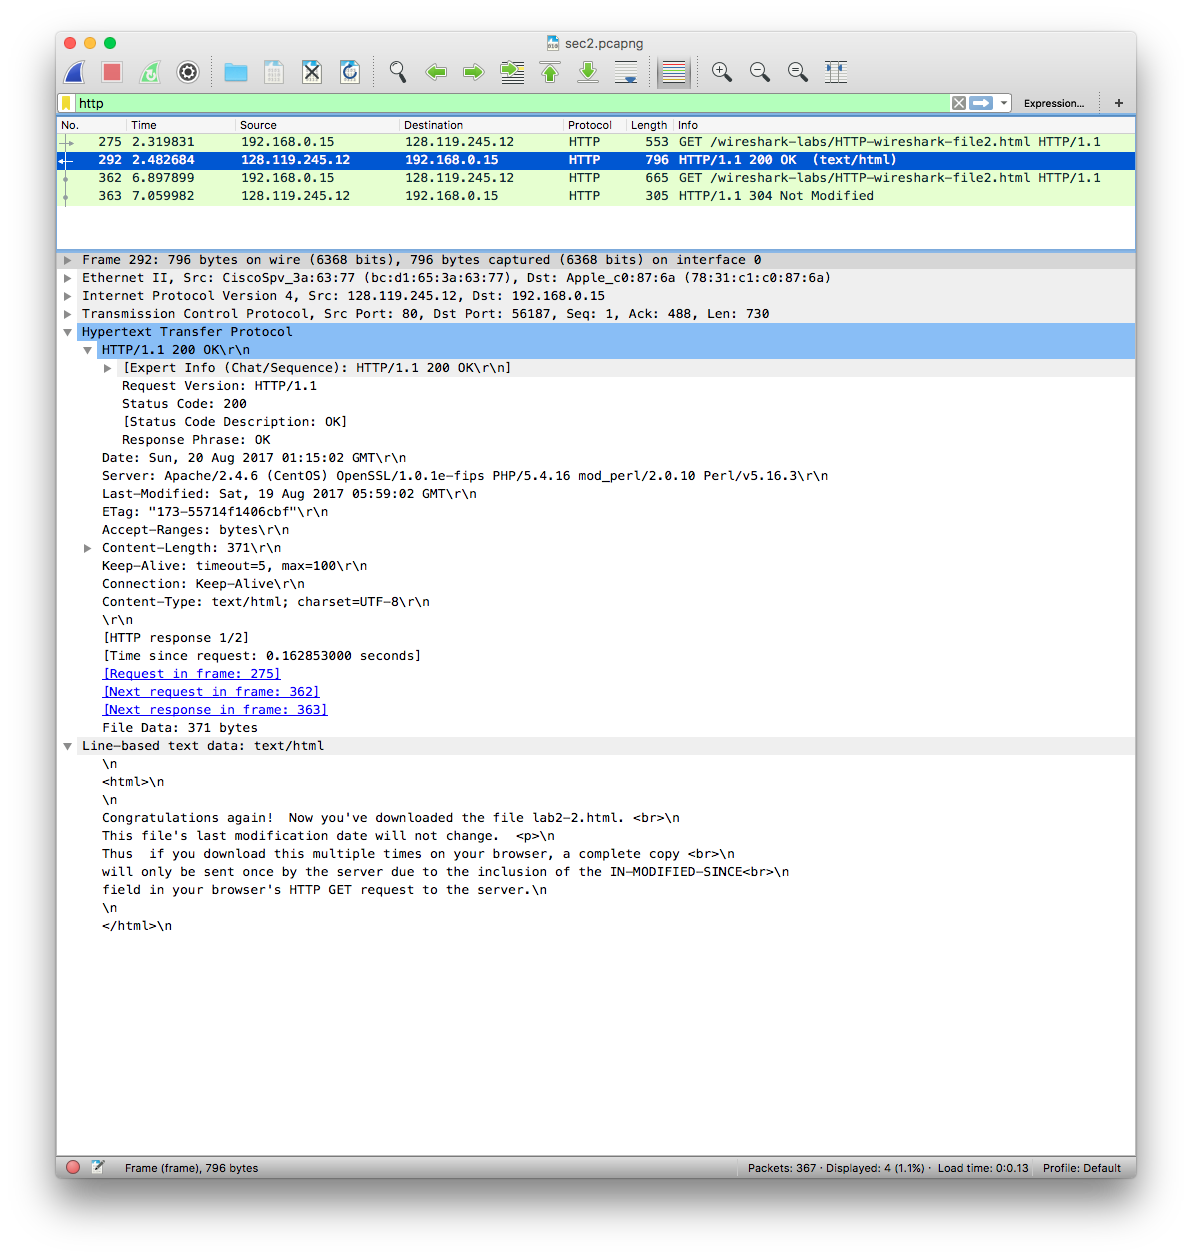
\includegraphics[width=\textwidth]{02-response_1}
		\end{figure}
		
	\item
		\textit{Now inspect the contents of the second HTTP GET request from your browser to the
server. Do you see an “IF-MODIFIED-SINCE:” line in the HTTP GET? If so, what
information follows the “IF-MODIFIED-SINCE:” header?}
		\par Yes, the information that followed the “IF-MODIFIED-SINCE:” header was the data it was modified `If-Modified-Since: Sat, 19 Aug 2017 05:59:02 GMT'.
	
		\begin{figure}[H]
		\centering
		\caption{Second Request (Section 2)}
		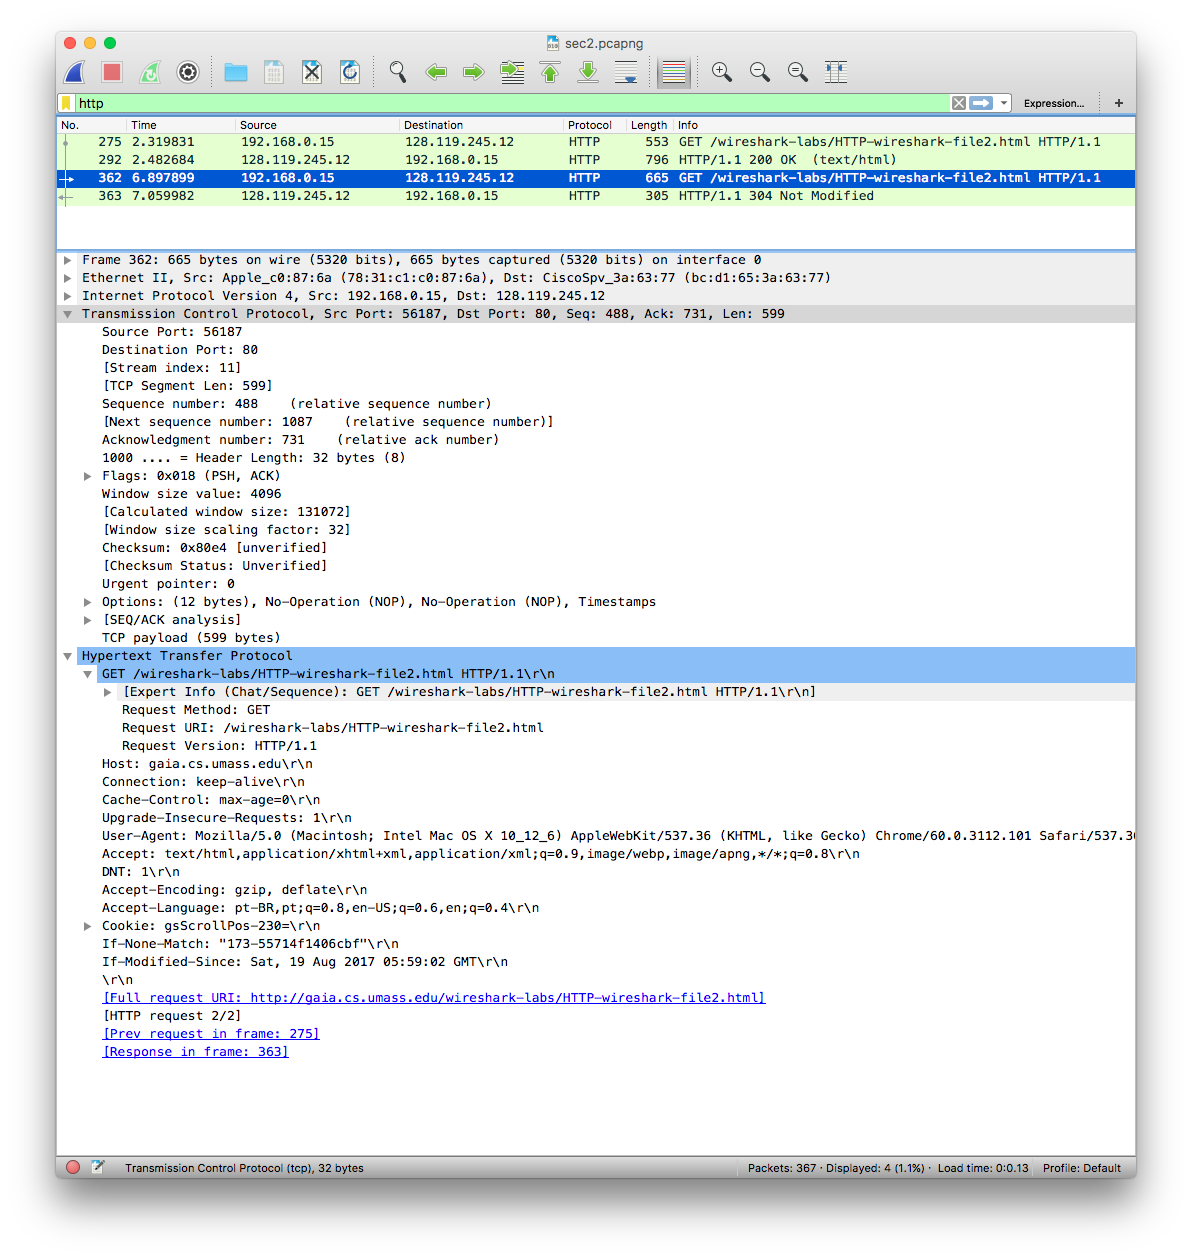
\includegraphics[width=\textwidth]{02-request_2}
		\end{figure}
		
	\item
		\textit{What is the HTTP status code and phrase returned from the server in response to this
second HTTP GET? Did the server explicitly return the contents of the file? Explain.}
		\par Status Code: 304 [Status Code Description: Not Modified]
		\par The server doesn't return the contents of the file because the information was previously cached by the browser after the first request.

		\begin{figure}[H]
		\centering
		\caption{Second Response (Section 2)}
		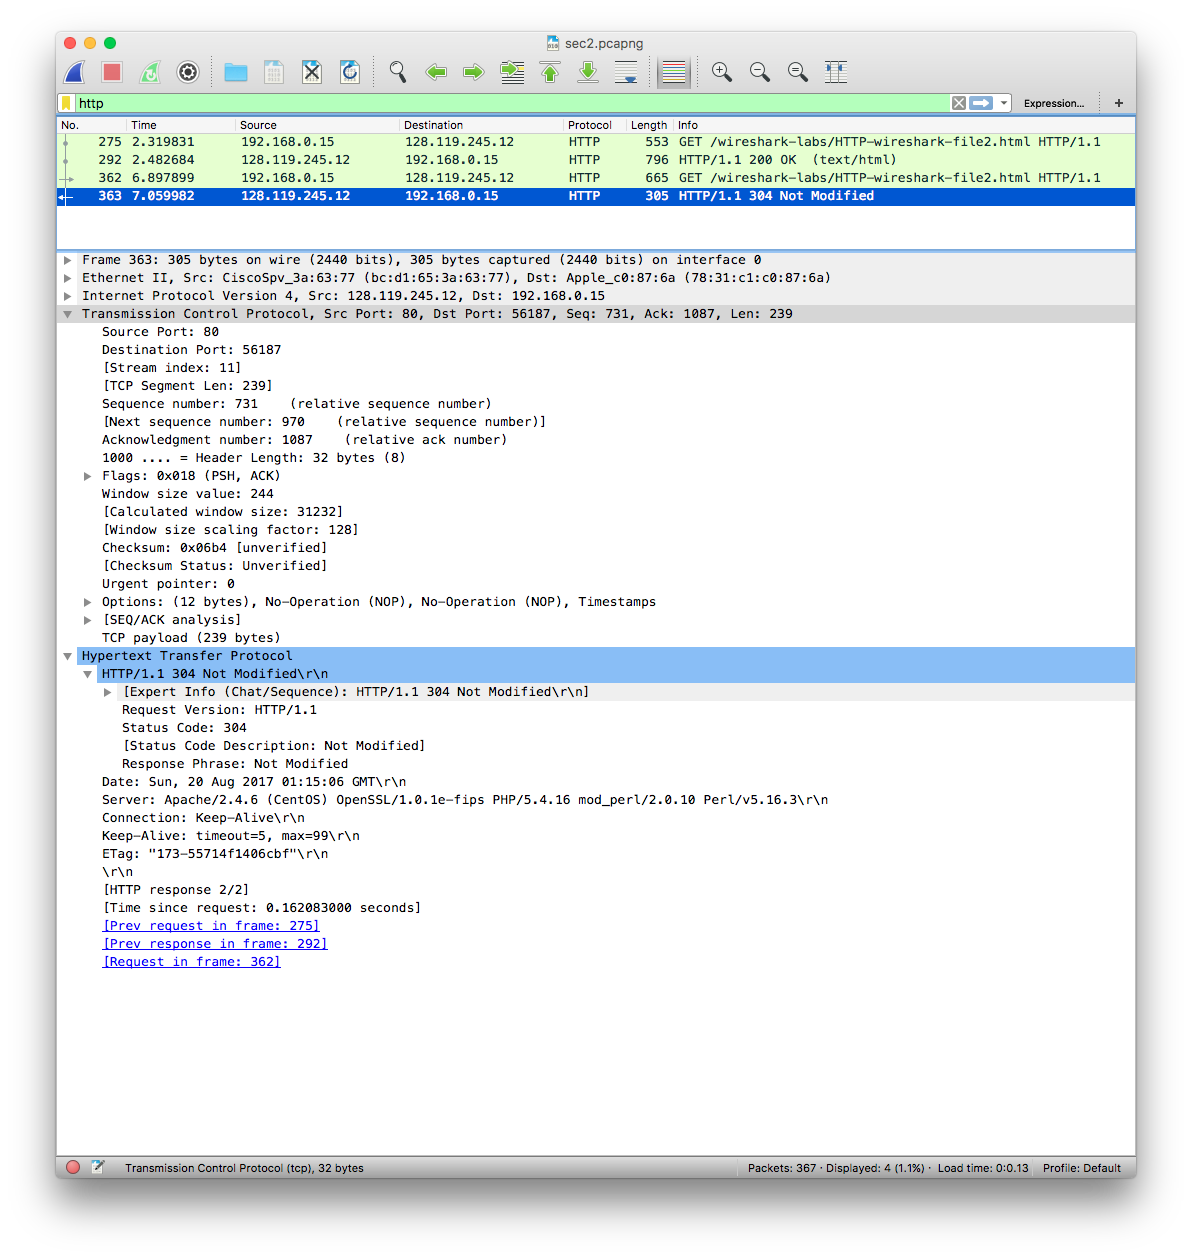
\includegraphics[width=\textwidth]{02-response_2}
		\end{figure}

\end{itemize}

% 3. Retrieving Long Documents
\section{Retrieving Long Documents}

\begin{figure}[H]
\centering
\caption{Request (Section 3)}
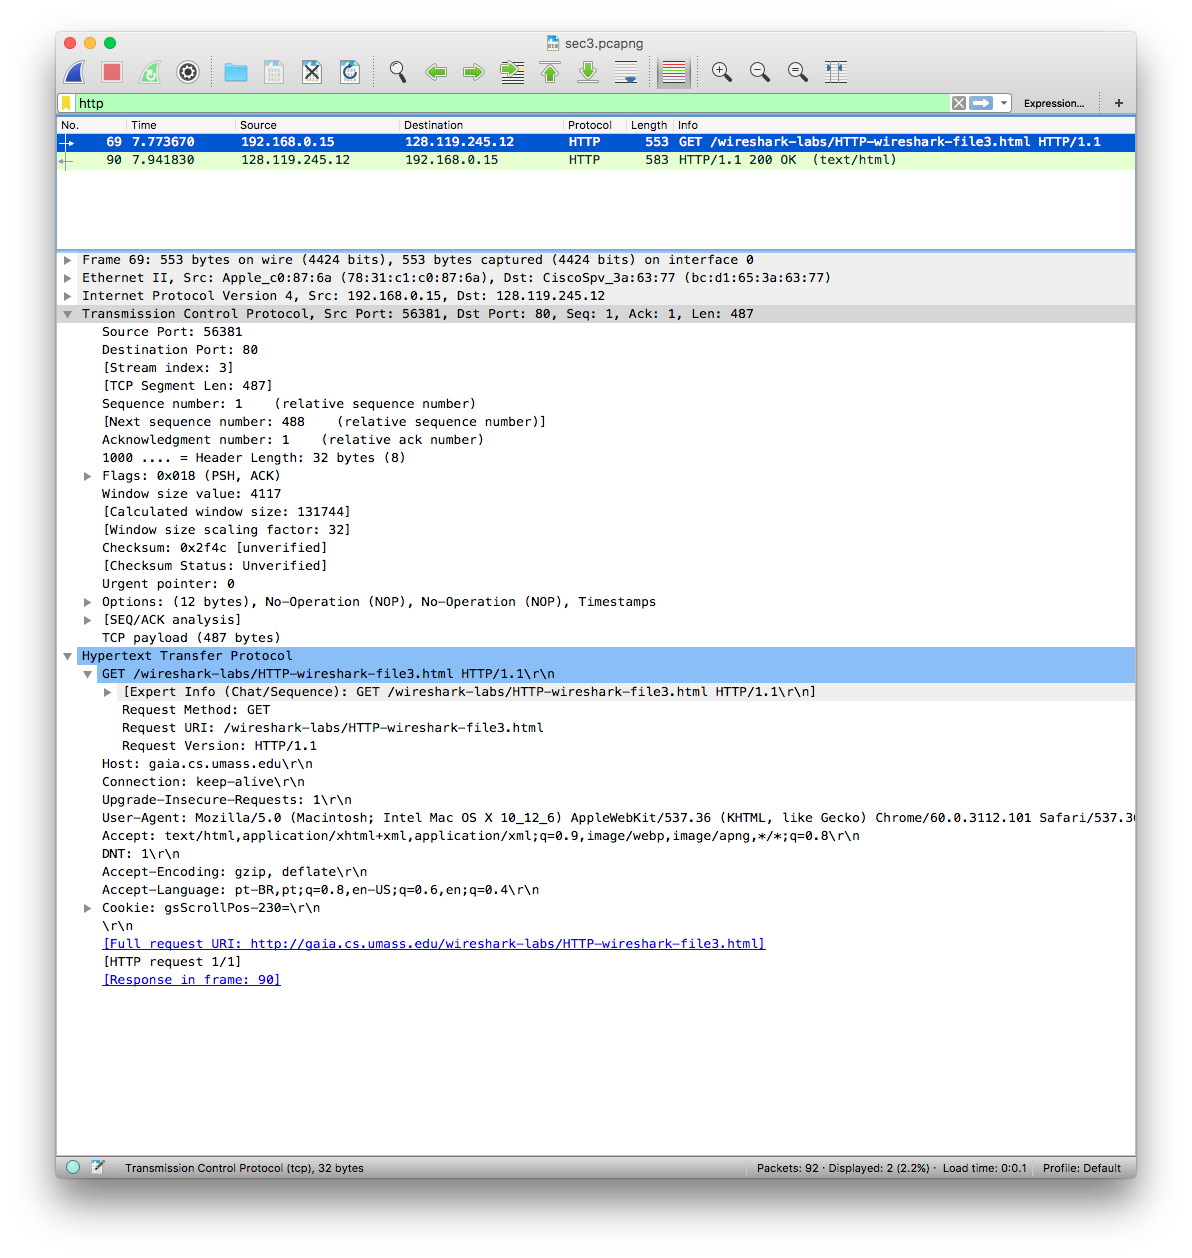
\includegraphics[width=\textwidth]{03-request}
\end{figure}

\begin{figure}[H]
\centering
\caption{Response (Section 3)}
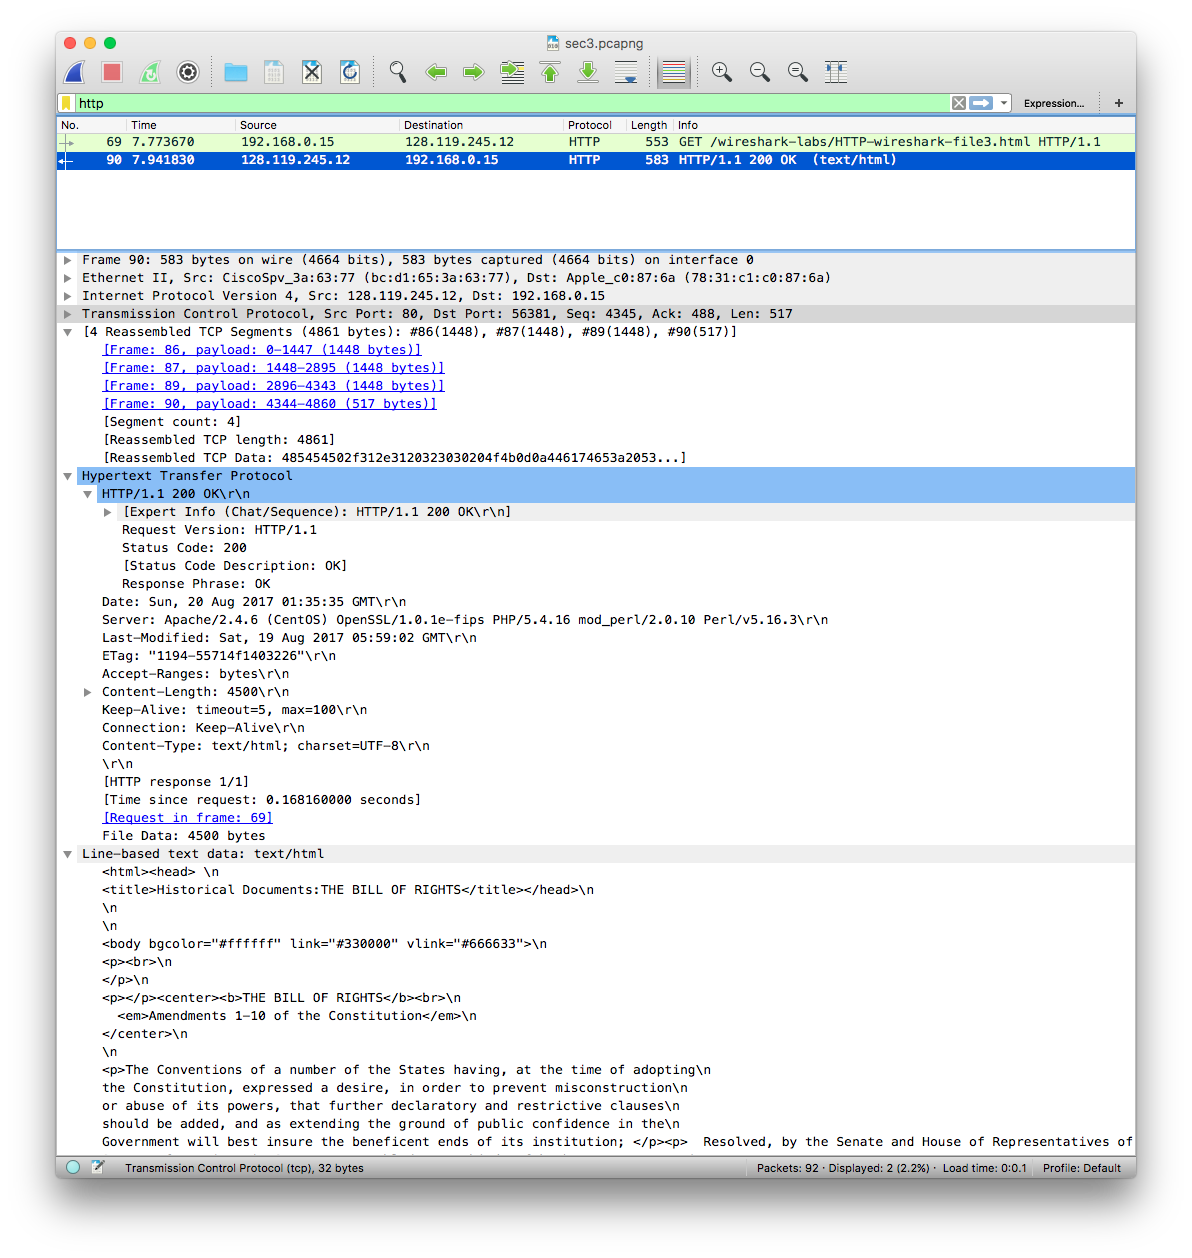
\includegraphics[width=\textwidth]{03-response}
\end{figure}

\pagebreak

\begin{itemize}
	\setlength\itemsep{.5cm}

	\item
		\textit{How many HTTP GET request messages did your browser send? Which packet number
in the trace contains the GET message for the Bill or Rights?}
		\par A single HTTP GET request was sent. Packet number 69 contained the GET message for the Bill of Rights.
		
	\item
		\textit{Which packet number in the trace contains the status code and phrase associated with
the response to the HTTP GET request?}
		\par Packet number 90 contained the response to the request.
		
	\item
		\textit{What is the status code and phrase in the response?}
		\par Status Code: 200 [Status Code Description: OK]
		\par Response Phrase: OK

	\item
		\textit{How many data-containing TCP segments were needed to carry the single HTTP
response and the text of the Bill of Rights?.}
		\par 4 TCP segments were needed to carry the HTTP response.
		

\end{itemize}

% 4. HTML Documents with Embedded Objects
\section{HTML Documents with Embedded Objects}

\begin{figure}[H]
\centering
\caption{Request (Section 4)}
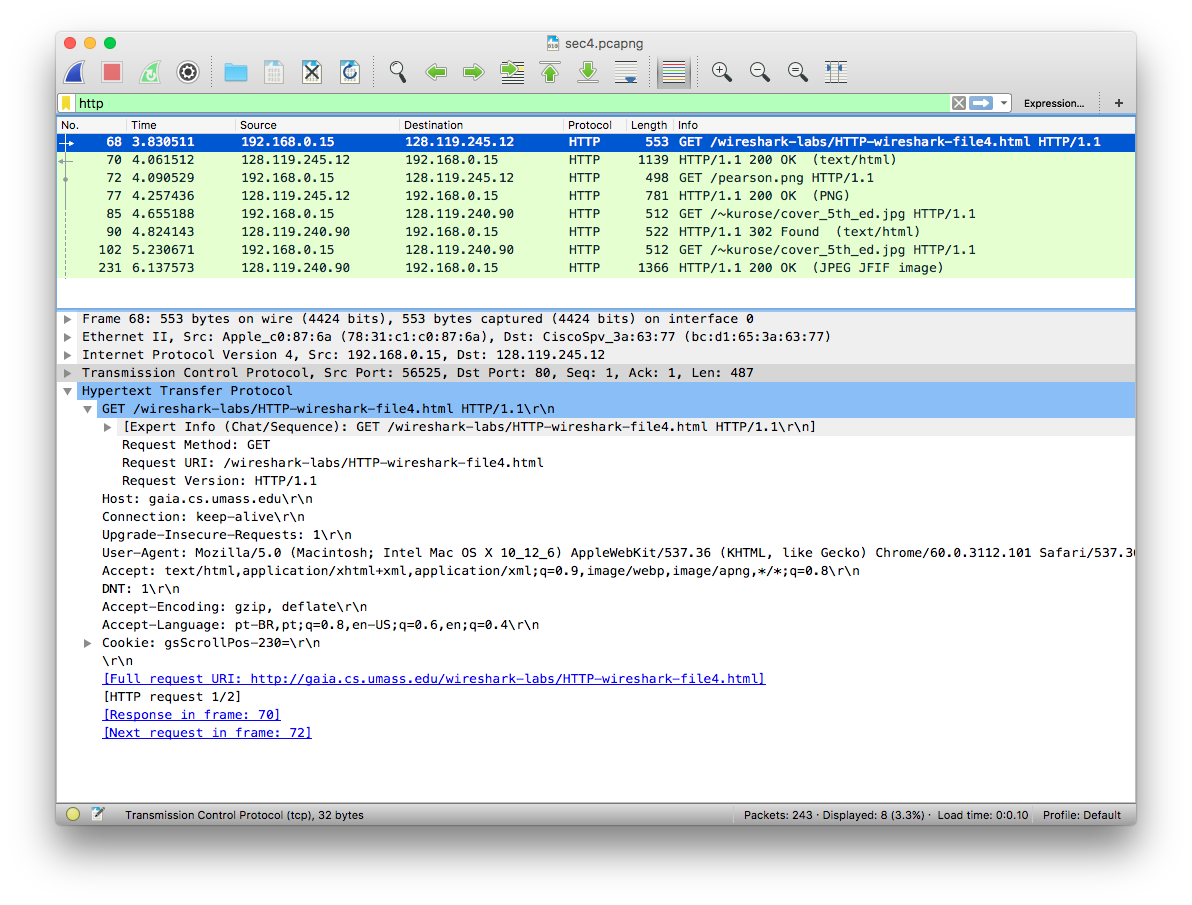
\includegraphics[width=\textwidth]{04-request}
\end{figure}

\begin{itemize}
	\setlength\itemsep{.5cm}

	\item
		\textit{How many HTTP GET request messages did your browser send? To which Internet
addresses were these GET requests sent?}
		\par 4 HTTP GET requests were sent. Each one of the following addresses received two GET requests: 128.119.245.12 and 128.119.240.90.
		
	\item
		\textit{Can you tell whether your browser downloaded the two images serially, or whether they
were downloaded from the two web sites in parallel? Explain.}
		\par The browser downloaded them serially because each request received a response before a new request was made.

\end{itemize}

% 5. HTTP Authentication
\section{HTTP Authentication}
		
\begin{itemize}
	\setlength\itemsep{1cm}

	\item
		\textit{What is the server’s response (status code and phrase) in response to the initial HTTP
GET message from your browser?}
	 \par Status Code: 401 - Response Phrase: Unauthorized
	 
	 	\begin{figure}[H]
		\centering
		\caption{First Response (Section 5)}
		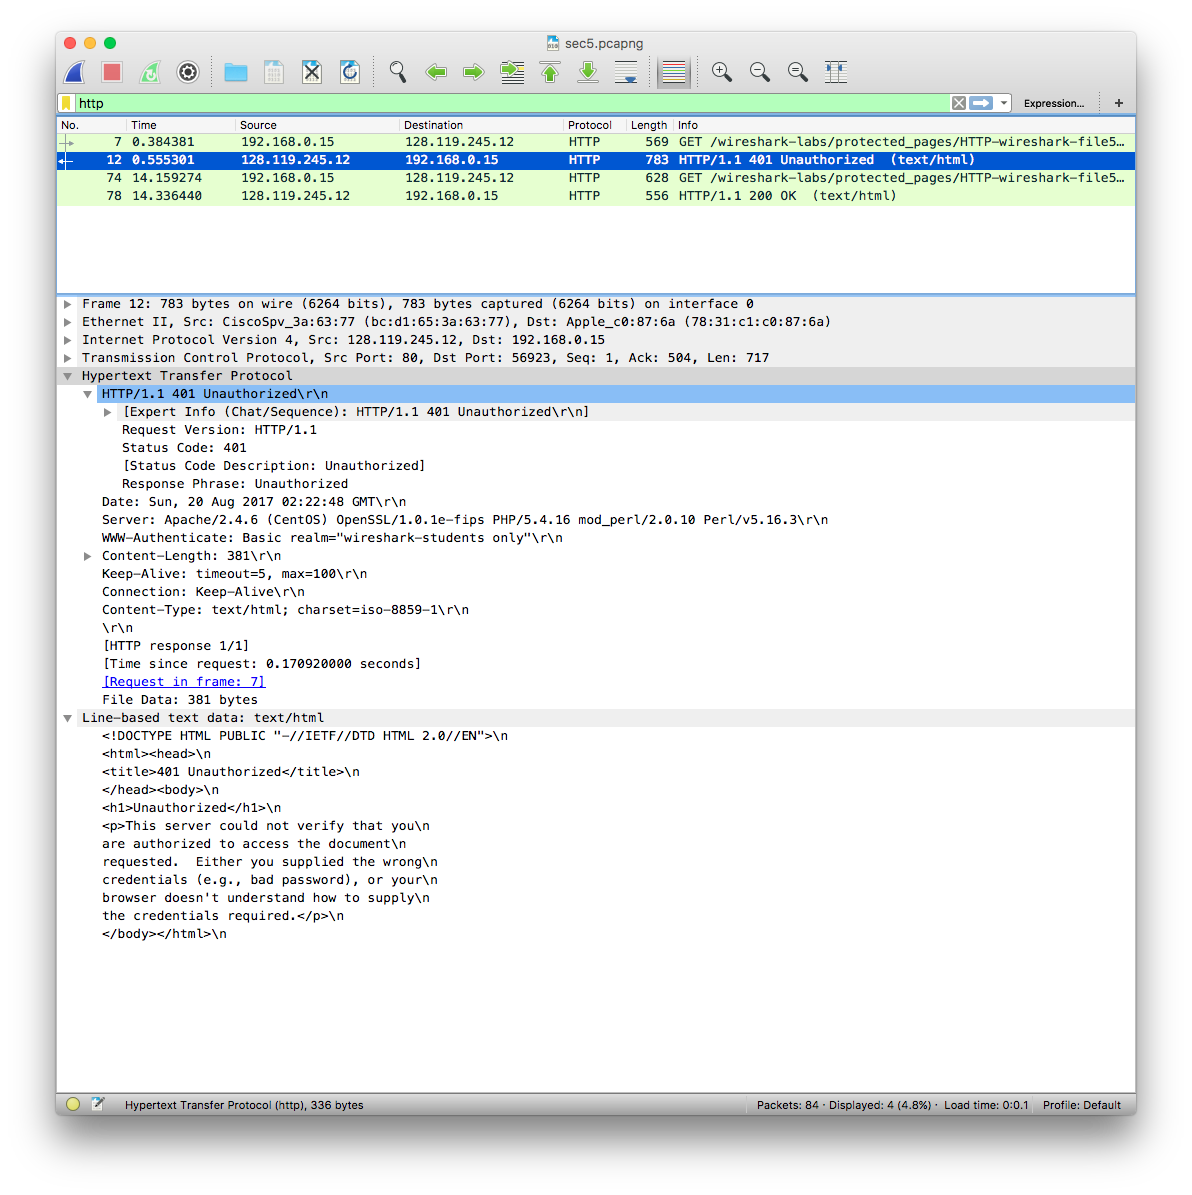
\includegraphics[width=\textwidth]{05-response_1}
		\end{figure}
		
	\item
		\textit{When your browser’s sends the HTTP GET message for the second time, what new
field is included in the HTTP GET message?}
		\par `Authorization' is the new field included. This new field provides the credentials (username and password).

	 \begin{figure}[H]
		\centering
		\caption{Second Request (Section 5)}
		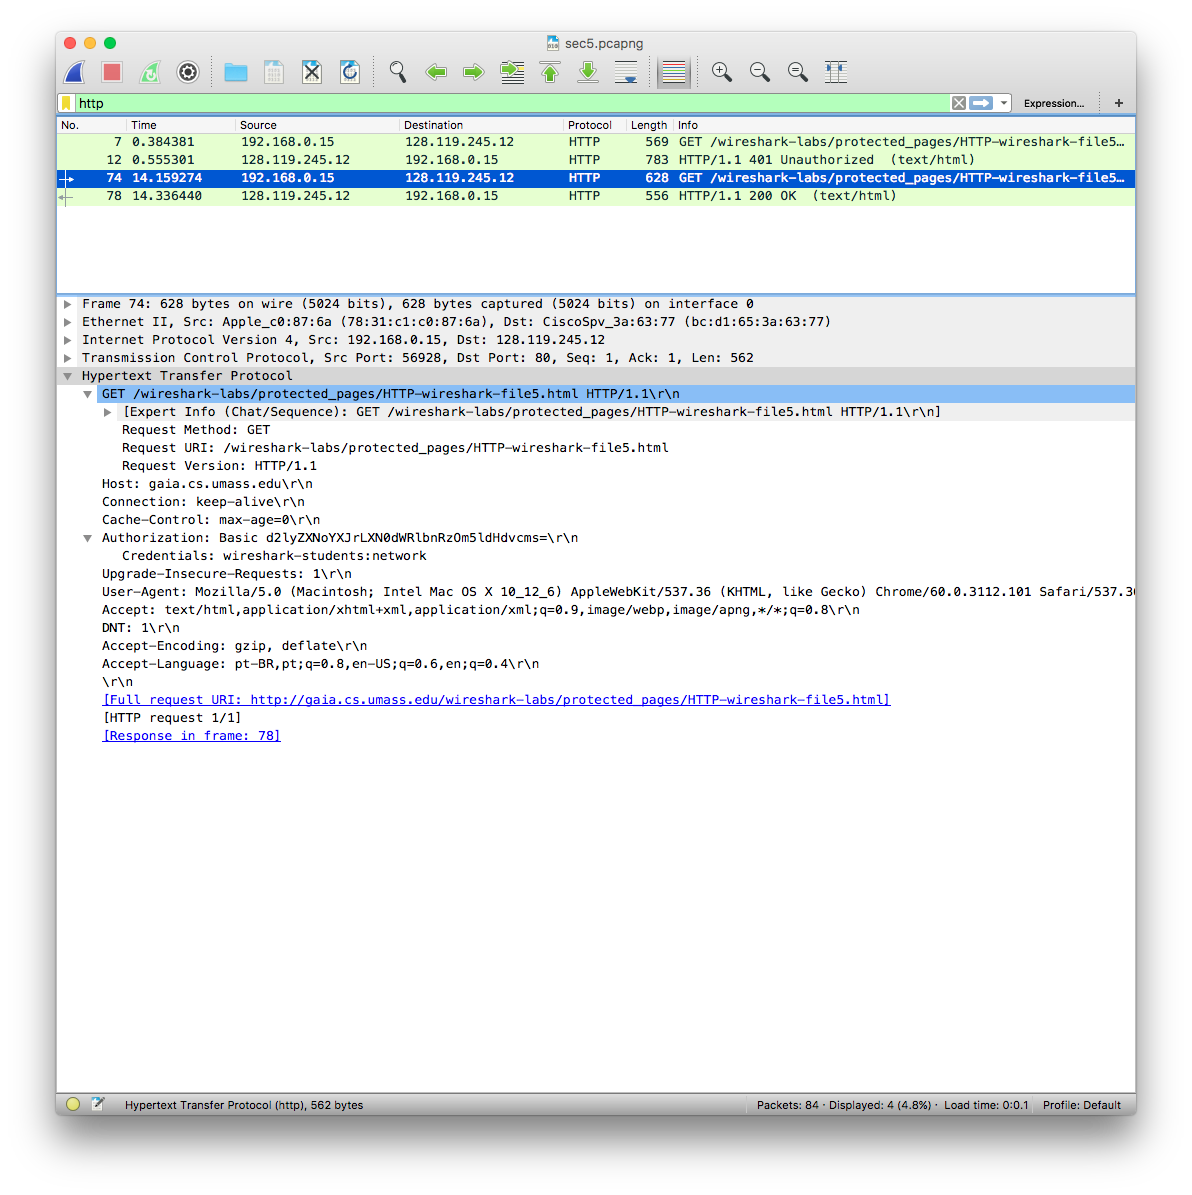
\includegraphics[width=\textwidth]{05-request_2}
		\end{figure}

\end{itemize}

\end{document}
